\documentclass[output=paper,colorlinks,citecolor=brown,draft]{langscibook}
\ChapterDOI{10.5281/zenodo.15006599}

\author{Hedwig G. Sekeres\orcid{0000-0003-0213-0805}\affiliation{University of Groningen} and Martijn Wieling\orcid{0000-0003-0434-1526}\affiliation{University of Groningen} and Remco Knooihuizen\orcid{0000-0002-2885-6359}\affiliation{University of Groningen}}
\title{A cognitive geographic approach to dialectology: Cognitive distance as a predictor for perceptual dialect distance}
\abstract{In this study, we explain perceptual dialect differences using both geographic distance and a different type of distance that is commonly used in the field of cognitive geography. Cognitive geography is based on the assumption that an individual's mental representation of their environment has a greater effect on their behaviour than the actual environment \citep{montello_behavioral_2018}. A commonly used metric in cognitive geography is the cognitive distance: the geographic distance between two places as estimated by an individual \citep{montello_measurement_1991}. This study also introduces the use of cognitive distances into dialect research and investigates whether these mental representations of space can serve as an explanatory variable in dialectology.

Nearly 800 participants from the north of the Netherlands provided cognitive distances between the place where they grew up and seven other locations in the same region. They also rated the similarity of dialect recordings from these locations to the dialect of the location where they grew up. A linear mixed-effects regression model was built to predict perceptual dialect distance from both cognitive distance and geographic distance. The resulting model indicates that geographic distance is more predictive of perceptual dialect distance than cognitive distance. There was also a significant interaction between cognitive and geographic distance. Cognitive distance is more predictive of perceptual dialect distance when geographic distance is short than when geographic distance is long. Furthermore, an exploratory analysis revealed that gender and proficiency in the participants' local dialect were predictive of perceptual dialect distance. Our findings indicate that cognitive distance can be used to explain dialect variation, especially when the area under investigation is small, and consequently that the framework of cognitive geography can be usefully employed in dialectological research.}

%move the following commands to the "local..." files of the master project when integrating this chapter
% % \usepackage{tabularx}
% % \usepackage{langsci-optional}
% % \usepackage{langsci-gb4e}
% % \usepackage{tipa}
% % \bibliography{localbibliography}
% % \newcommand{\orcid}[1]{}

\IfFileExists{../localcommands.tex}{
   \addbibresource{../localbibliography.bib}
   \usepackage{tabularx,multicol}
%\usepackage{multirow}
\usepackage{subcaption}
\usepackage{url}
\urlstyle{same}

\usepackage{datetime}
\usepackage{enumitem}
\usepackage{langsci-optional}
\usepackage{langsci-lgr}
\usepackage{langsci-branding}

\usepackage{longtable}
\usepackage{xltabular}
\usepackage[linguistics, edges]{forest}
\usepackage{pgfplots}
\pgfplotsset{compat=1.18}
\usetikzlibrary{patterns, tikzmark}
\usepackage{pgfplotstable}
\usepgfplotslibrary{colorbrewer}
\usepackage{listings}
\lstset{basicstyle=\ttfamily,keywordstyle=\normalfont,language=,breaklines=true}

\usepackage{siunitx}
\sisetup{group-digits=none, detect-all=true}

\usepackage{langsci-gb4e}

   \makeatletter
\let\thetitle\@title
\let\theauthor\@author
\makeatother

% Use this Chinese font shipped with TeX Live instead of Source Han, because
% it is more portable/leightweight. Install the "fandol" package from CTAN to
% automatically get this font.
\newfontfamily{\ChineseFandolSong}{FandolSong-Regular.otf}

   %% hyphenation points for line breaks
%% Normally, automatic hyphenation in LaTeX is very good
%% If a word is mis-hyphenated, add it to this file
%%
%% add information to TeX file before \begin{document} with:
%% %% hyphenation points for line breaks
%% Normally, automatic hyphenation in LaTeX is very good
%% If a word is mis-hyphenated, add it to this file
%%
%% add information to TeX file before \begin{document} with:
%% %% hyphenation points for line breaks
%% Normally, automatic hyphenation in LaTeX is very good
%% If a word is mis-hyphenated, add it to this file
%%
%% add information to TeX file before \begin{document} with:
%% \include{localhyphenation}
\hyphenation{
    a-na-ly-sis
    ap-proach-es
    ar-che-o-log-i-cal
    Ar-khan-gelsk
    be-schrei-ben
    Buch-holtz
    Che-lya-binsk
    con-so-nant
    dia-lect
    dia-lect-ology
    Di-a-lekt-for-schung
    Dia-lekt-for-schung
    East-pha-lian
    För-der-ung
    Ge-mein-schaft-lich-keits-ent-wür-fe
    his-tor-i-cal
    Hok-kai-do
    ja-pa-nese
    Ja-pa-nese
    Ka-go-shi-ma
    Ka-li-nin-grad
    Knja-zev
    Ma-kro-be-reich
    Ma-lay-sia
    mor-pho-log-i-cal
    Mos-cow
    Nef-te-yu-gansk
    non-mobile
    nu-cle-ar
    ös-ter-rei-chi-sche
    par-a-digm
    per-zep-ti-ons-lin-gu-is-ti-sche
    plu-ri-zen-tri-schen
    quick-ly
    Reich
    Sax-on
    Schrö-der
    sear-ching
    ste-reo-type
    strength-en-ing
    strong-est
    Stutt-gart
    su-pra-seg-men-tal
    teach-er
    to-po-gra-phy
    To-ron-to
    tra-di-tion-al
    ul-ti-mate-ly
    Um-gangs-spra-che
    Volks-kun-de
    vor-zu-stel-len
    wheth-er
    Wie-sing-er
    with-in
    Wort-at-las
}

\hyphenation{
    a-na-ly-sis
    ap-proach-es
    ar-che-o-log-i-cal
    Ar-khan-gelsk
    be-schrei-ben
    Buch-holtz
    Che-lya-binsk
    con-so-nant
    dia-lect
    dia-lect-ology
    Di-a-lekt-for-schung
    Dia-lekt-for-schung
    East-pha-lian
    För-der-ung
    Ge-mein-schaft-lich-keits-ent-wür-fe
    his-tor-i-cal
    Hok-kai-do
    ja-pa-nese
    Ja-pa-nese
    Ka-go-shi-ma
    Ka-li-nin-grad
    Knja-zev
    Ma-kro-be-reich
    Ma-lay-sia
    mor-pho-log-i-cal
    Mos-cow
    Nef-te-yu-gansk
    non-mobile
    nu-cle-ar
    ös-ter-rei-chi-sche
    par-a-digm
    per-zep-ti-ons-lin-gu-is-ti-sche
    plu-ri-zen-tri-schen
    quick-ly
    Reich
    Sax-on
    Schrö-der
    sear-ching
    ste-reo-type
    strength-en-ing
    strong-est
    Stutt-gart
    su-pra-seg-men-tal
    teach-er
    to-po-gra-phy
    To-ron-to
    tra-di-tion-al
    ul-ti-mate-ly
    Um-gangs-spra-che
    Volks-kun-de
    vor-zu-stel-len
    wheth-er
    Wie-sing-er
    with-in
    Wort-at-las
}

\hyphenation{
    a-na-ly-sis
    ap-proach-es
    ar-che-o-log-i-cal
    Ar-khan-gelsk
    be-schrei-ben
    Buch-holtz
    Che-lya-binsk
    con-so-nant
    dia-lect
    dia-lect-ology
    Di-a-lekt-for-schung
    Dia-lekt-for-schung
    East-pha-lian
    För-der-ung
    Ge-mein-schaft-lich-keits-ent-wür-fe
    his-tor-i-cal
    Hok-kai-do
    ja-pa-nese
    Ja-pa-nese
    Ka-go-shi-ma
    Ka-li-nin-grad
    Knja-zev
    Ma-kro-be-reich
    Ma-lay-sia
    mor-pho-log-i-cal
    Mos-cow
    Nef-te-yu-gansk
    non-mobile
    nu-cle-ar
    ös-ter-rei-chi-sche
    par-a-digm
    per-zep-ti-ons-lin-gu-is-ti-sche
    plu-ri-zen-tri-schen
    quick-ly
    Reich
    Sax-on
    Schrö-der
    sear-ching
    ste-reo-type
    strength-en-ing
    strong-est
    Stutt-gart
    su-pra-seg-men-tal
    teach-er
    to-po-gra-phy
    To-ron-to
    tra-di-tion-al
    ul-ti-mate-ly
    Um-gangs-spra-che
    Volks-kun-de
    vor-zu-stel-len
    wheth-er
    Wie-sing-er
    with-in
    Wort-at-las
}

   \boolfalse{bookcompile}
   \togglepaper[23]%%chapternumber
}{}
\shorttitlerunninghead{A cognitive geographic approach to dialectology}

% #1: sorting key, #2: prefix for citation, #3: prefix for bibliography
\DeclareRobustCommand{\VAN}[3]{#3} % set up for citation

\begin{document}
\graphicspath{{figures/sekeres}}
\maketitle
\label{chap:sekeres}

\section{Introduction}
In dialectology, space has historically been treated for the most part as a blank canvas on which linguistic (and sometimes social) information is visualised. This treatment of space has been criticised as too one-dimensional and dismissive of findings from different subdisciplines of geography \citep[e.g.,][]{britain_space_2013}, but as of yet only a small amount of research has been done in which a broader consideration of space in dialectology is taken. Perceptual dialectology to some degree forms an exception to this, as methods from the field of cultural geography have been adapted for dialect research by perceptual dialectologists, most notably \citet[e.g.,][]{preston_perceptual_1981, preston_handbook_1999}. However, while cultural geography concerns itself with the spatial distribution of culture \citep{anderson_handbook_2003} and in the case of perceptual dialectology, language and language attitudes, the ways in which space itself can influence attitudes and behaviour are not its main focus. An analysis of this relationship forms an interesting addition to the analysis of dialect variation. One field that does concern itself with this particular relationship is \textit{cognitive} (as opposed to the aforementioned \textit{cultural}) geography, which focuses on the mental representations of space that people have and how these influence their behaviour. This study introduces the cognitive geographic measure of \textit{cognitive distances} into dialect research and investigates whether these mental representations of space can serve as an explanatory variable in dialectology. Specifically, we do this by investigating whether including cognitive distance, in addition to geographic distance, leads to better predictions of perceptual dialect distance in the Gronings dialect area.

\section{Background}
\subsection{Traditional notions of space in dialectology}
In traditional dialectology, space is usually represented by a map on which language variation is presented. The first dialect maps were often representations of the geographical variation of one word or a single linguistic feature, where different variants of that word or the different variants of the feature were written on the map at their respective locations \citep{rabanus_dialect_2017}. Although these maps were detailed and precise, they were not very insightful as it can be difficult to discover patterns in the spatial distribution of words. Later dialect maps made use of points with different shapes or colours to signify the different variants that were present and provided a more easily accessible overview of the geographic patterns of language variation. A different type of dialect map uses isoglosses to signal borders in dialects or languages, usually between different variants of a feature. Maps consisting of bundles of isoglosses made it easier to distinguish between areas in which related variants are used \citep{rabanus_dialect_2017}. Although space plays an important role in these visualisation techniques, it is for the most part treated as a blank canvas and a recipient for linguistic (and sometimes extra-linguistic) information. Some conclusions about spatial patterns other than geographic distance can be based on the administrative and geographic features that are sometimes present on these maps, but not in a systematic manner. This is, of course, not to say that social, historical and political patterns that are themselves spatially stratified have not been used to explain (spatial) variation in dialects. In Germany and the Netherlands, in particular, expansiological dialectology has been influential in offering alternatives to explaining spatial patterns that are not purely geographical by including information on communicative patterns \citep{goossens_geschiedenis_1977}.
\largerpage
Space itself as an explanatory variable had not been taken into account in dialectology until the early 1970s, when different models of the diffusion of language change were proposed. These new models of diffusion were a criticism of the wave model \citep{bailey_variation_1973}, which proposed that new variants moved through space more or less in a straight line, spreading from one location to the next on the basis of proximity. The most prominent example of these new models is the gravity model \citep{trudgill_linguistic_1974}, which proposed that language change does not spread through space evenly but that new variants take hold in large population centres first and then spread to rural areas. In the gravity metaphor that is used, urban centres exert a certain gravitational pull on new variants, pulling them towards themselves before they reach rural areas. In this model, social aspects of space are granted more importance than in the wave model as it takes into account other (non-linguistic) phenomena that are stratified across space and that influence both space itself and human (linguistic) behaviour. Research on the spread of language change often found conflicting results. One study on Oklahoma dialects found, for example, that change from above followed a different spatial pattern, spreading from urban to rural, than change from below, which spread from rural to urban \citep{bailey_variation_1973, labov_mechanisms_1965}. Here we find that dialectology really starts to engage more with space and spatial patterns, as the interactions between linguistic and spatial phenomena are researched. In the Netherlands, a dialectometric study investigating the use of the gravity model in the Netherlandic Low Saxon language area found patterns of diffusion that were the opposite of what the gravity model would predict \citep{nerbonne_dialectometric_2005}. However, that study did not differentiate different types of features, so no interaction between spatial and linguistic patterns could be found. 
\newpage
Some special attention regarding the interaction between language and space is merited by the field of perceptual dialectology as it has engaged with methods from different geographic subdisciplines from an early stage. Whereas traditional dialectology concerns itself with dialects as described by linguists, the field of perceptual dialectology investigates the attitudes and beliefs that non-linguists have about dialects and dialect variation \citep{preston_handbook_1999}. 

The field of perceptual dialectology came into existence more or less simultaneously in Japan and the Netherlands, with accounts differing on the birthplace of the field \citep{montgomery_perceptual_2011}. In the Netherlands, the so-called \textit{pijltjesmethode} (or `little-arrow method') was developed. In this approach, participants were asked to indicate in which locations the dialect was the same or very similar to 
their own dialect. This information was visualised on maps with small arrows that indicated which areas were seen as similar by the participants. These maps were then compared with dialect maps based on known dialect differences and isoglosses in order to assess whether the participants' perception of dialects matched the 
actual dialect situation. For many areas, this was the case although interesting differences between production and perception of dialect differences arose as well \citep{weijnen_grenzen_1946}. In Japan, dialectologists took a similar approach in which they asked participants to rate the similarity of their dialect to other dialects on a continuum. The results of this task were visualised on a map in which lines were drawn to signify the different 
perceptual areas \citep{sibata_consciousness_1999}. Results from these studies differed more starkly from the dialect areas that were traditionally distinguished, and gave rise to the investigation of different components of language variation in dialectology, such as pitch accent \citep{montgomery_perceptual_2011}. 

From the 1980s onwards, the field of perceptual dialectology underwent great development, when Dennis Preston incorporated mental maps from the field of cultural geography in dialectology \citep{montgomery_perceptual_2011, preston_perceptual_1981}. In cultural geography, mental maps have been used from the 1960s onwards to visualise the mental representations that people have of space \citep{lynch_image_1964, portugali_history_2018}. This is usually done by prompting participants to draw a map of a certain area as they remember or perceive it, sometimes with a specific goal in mind such as to draw important landmarks or their commute to work. Mental maps provide insight into the places people find important and how they believe these places relate to each other \citep{gould_mental_1974}. Preston adapted the mental maps to dialectological research and created the so-called \textit{draw-a-map task}. In this task, participants are asked to indicate on a map where they would locate certain speech patterns, and sometimes also which types of people they associate with these patterns. With the introduction of this task, space started to play an integral role in perceptual dialectology as the visualisation of linguistic information is not only done by researchers after the linguistic data has been collected, but the participants themselves are also required to think about dialects in space. In this way, linguistic data are generated in a manner that is inherently more spatially oriented. However, as the draw-a-map task was borrowed from the field of cultural geography rather than cognitive geography, the mental representations of space itself are not used as an explanatory variable in this type of research. As with the maps made in traditional dialectology, space is rather a blank canvas on which linguistic and -- in this case -- social data are visualised, and not a factor that is to be taken into consideration on its own. One notable addition to the analysis of these maps is the use of the cultural prominence of locations by \citet{montgomery_effect_2012}. He found that areas that were drawn by participants on their dialect maps had almost without exception undergone an increase in cultural prominence based on the number of mentions in two newspapers per head of population. Although the participants themselves in this case did not give indications of the cultural prominence of regions, this approach does acknowledge that properties of a region can affect people's dialect perception. 

Next to the draw-a-map task, Preston developed and adapted several other techniques for perceptual dialectological research. One such technique is asking participants to rate the difference between a given dialect and the dialect spoken at the place where the participant grew up. This measure, also called the \textit{perceptual dialect distance}, is also employed in our study. Other methods introduced by Preston are the collection of non-linguists' ratings of the correctness and/or pleasantness of dialects, asking participants to identify a dialect and to link it to a geographic location, and conducting interviews to gather qualitative data on non-linguists' attitudes and beliefs, for example by asking them about the previous tasks or to talk about characteristics of the speakers of certain variants \citep{preston_handbook_1999}. 

Research in perceptual dialectology actively engages with space in the sense that participants in a draw-a-map task or an interview are asked to think about language spatially. However, the variables used to explain why participants hold certain attitudes or give certain judgments are typically social, not spatial. Treating space itself as an explanatory variable that encompasses more than merely geographic distance is still relatively rare. This omission has been criticised in the field of dialectology in general: ``Space has largely been treated as an empty stage on which sociolinguistic processes are enacted. It has been unexamined, untheorised and its role in shaping and being shaped by variation and change untested'' \citep[471]{britain_space_2013}. There are developments in this regard, with several authors pointing out the importance of perceptual space in language variation \citep[e.g.][]{britain_conceptualizations_2011, Preston2010}, but to our knowledge this has not yet resulted in studies in which perceptual space is quantified and included as a variable. 

\subsection{Alternative notions of space in dialectology}
One of the most frequently used alternatives for geographic (as-the-crow-flies) distance in dialectology is travel distance, expressed as the number of kilometres one would need to travel to get from location A to location B. The advantage of using travel distance over geographical distance is that it provides researchers with more insight into possible contact situations. Using travel distance as a way to incorporate this geographic information in dialectology was done, for example, by \citet{van_gemert_het_2002}, and later adapted in the form of travel times by \citet{gooskens_norwegian_2004}. Gooskens found that dialect distances in Norway correlated more strongly with historical travel times than with simple Euclidean distances, which was explained by the amount of contact that dialects historically had, due to the amount of time that travel would take \citep{gooskens_norwegian_2004}. The use of both travel distances and travel times in dialectological research has further successfully been demonstrated in a study on Japanese dialects \citep{jeszenszky_japanese_2019}, in which an increase in travel distance and travel time correlated positively with an increase in dialect distance. Although neither travel distance nor travel time outperformed geographic distance in this study (partly because of the difficulty to include travel over water), travel times are still a promising approach to incorporate both space itself and the \textit{experience} of space in dialectological research. Travel times in particular are suitable for this goal, as they relate to the way a journey is experienced: travelling 20 kilometers by car is experienced differently than travelling the same distance by foot. 

Next to travel distances and travel times, there are still other alternative notions of space used in dialectology that are more reflective of contact situations than geographic distance. In his study on the small clan-based Sui society in southwest China, \citet{stanford_one_2012} used the least cost distance between rice paddies instead of Euclidian or travel distances. He postulated that this distance measure forms a better reflection of mobility among the Sui people because it represents a more stable and historical social pattern than roads. The rice paddy distance explained dialect variation marginally but not significantly better than simple geographic distance \citep{stanford_one_2012}. Although the results of this study are not conclusive regarding the effects of using a different distance measure than geographic or travel distance, the study poses an interesting view on using a distance measure that more accurately reflects mobility patterns of a particular society. In recent years, more importance has been placed on the consideration of personal mobility in dialect research, although this interest does not necessarily translate into different types of distance measures. \citet{britain_space_2013}, for example, has argued for a more thorough investigation of mobility practices in border regions in order to understand why certain spatial patterns emerge in language use that are not easily explained by geography itself. Furthermore, a recent publication by \citet{JeszenszkyEtAl2024} proposes a personal mobility index for use in dialectological research. These developments offer a promising perspective in the future treatment of space in dialectology. 

\subsection{Cognitive geography}
In treating space for the most part as a combination of degrees of longitude and latitude, dialectological research does not take into account that people do not simply exist in space. They are also influenced by their spatial environment, and vice versa. One field that recognises this bi-directional relationship between people and their environment is cognitive geography. Like cultural geography, which has previously been employed in perceptual dialectological studies, cognitive geography is a subdiscipline of human geography, which concerns itself primarily with the relationship between humans and their environment. Although there is considerable overlap between cultural geography and cognitive geography, there are also important differences between these disciplines. Cultural geography mainly focuses on the spatial distribution of culture, identity and power dynamics \citep{anderson_handbook_2003}. Although researchers recognise that humans are influenced by their environment and vice versa, the cognitive processes that play a role in this influence are not the main object of study in the field. One of the most important characteristics of cognitive geography, on the other hand, is that it maintains that people's behaviour is influenced by their mental representations of their environment more than by the reality of their environment. This means that a person's perception of the distance between two places, for example, has more influence on their willingness to travel between these places than the actual distance. If they falsely believe the distance to be long, this mental representation of distance is more important than the fact that the distance is short. This relationship between mental representations of the environment and behaviour is the central object of study in cognitive geography \citep{montello_cognitive_2009, montello_behavioral_2018}. Other important characteristics of cognitive geography are (1) that the analysis is often disaggregate and focusses on the individual, (2) that the individual and the environment affect each other, and (3) that cognitive geographic research is inter- and multidisciplinary \citep{montello_behavioral_2018}. 

As it is impossible to directly access a person's cognition, cognitive geographers make use of several techniques to access cognition indirectly. One way of doing this is through so-called cognitive distances. Cognitive distances are the geographic distances between two places as estimated by an individual. In the field of cognitive geography, a distinction is made between cognitive and perceptual distances. Perceptual distances can only be estimated when the individual can see the places they have to estimate the distance to, such as a door within the same room or a tree that is visible some distance away. Cognitive distances, on the other hand, are used in situations in which the place that the individual has to estimate the distance towards is obscured from view \citep{montello_measurement_1991}, for example when estimating the distance to a building the participant is familiar with but that is not currently visible or the distance between two cities. It is important to note this distinction, as the distance estimates in our study are \textit{perceptual} when dialectology is concerned (participants were able to listen to audio recordings), but \textit{cognitive} when geography is concerned (participants were not able to see the locations). Cognitive distances can be used to quantify whether an individual overestimates or underestimates actual geographical distance. Over- or underestimation of geographic distance is dependent on many factors which are partly environmental, partly individual, and partly a mixture of the two \citep{qi_formal_2006}. The most important of the individual factors is familiarity, with an increase in familiarity causing a decrease in cognitive distance \citep{montello_measurement_1991}. For example, a study in which participants at different levels of familiarity with Sydney were tasked with providing distance estimates for locations within Sydney found that distance is generally overestimated, but that this overestimation is reduced by familiarity to a location \citep{day_urban_1976}. Related but slightly different is the notion that travel times are most predictive of cognitive distance, and that cognitive distance is mostly estimated on the basis of (perceived) travel times \citep{maceachren_travel_1980}. Other factors such as age, gender \citep{lawton_sex_2018} and individual differences in spatial cognition also play a role \citep{jenkins_cognitive_1992}. It is important to note that, although there are studies and theories on the underlying factors that influence or stand at the basis of cognitive distance, there is no real way of understanding what happens cognitively when someone makes an estimate of distance as any of the aforementioned (or other) factors could play a role. 

Although there is no research known to the authors in which the mental representations of space in the individual are used to explain linguistic phenomena, research in the opposite direction, i.e., using methods and frameworks from linguistics for explaining cognitive geographic phenomena, does exist. Typical examples would be the use of discourse analytic methods to assess wayfinding strategies and route descriptions \citep[e.g.,][]{holscher_would_2011} or the improvement of navigational software by using more human language \citep[e.g.,][]{baltaretu_improving_2015}. In these cases, language is not the object of research, but techniques from linguistics are used to access cognition which is then translated into conclusions about spatial cognition \citep[see][]{tenbrink_cognitive_2020}.

\subsection{The dialect landscape of Groningen and northern Drenthe}
The area under investigation, i.e., the province of Groningen and the northern part of the province of Drenthe, is located in the Low Saxon language area in the Netherlands. Low Saxon forms a dialect continuum that stretches from the East of the Netherlands into Germany and a small part of Denmark \citep{gooskens_cross-border_2009}. In the Netherlands, Low Saxon is a minority language that is recognised under part two of the European Charter for Regional or Minority Languages \citep{noauthor_europees_1998}. According to the most recent survey study, Low Saxon is spoken by roughly 75\% of the population in the Low Saxon areas in the Netherlands (i.e., the provinces of Groningen, Drenthe and Overijssel, the municipalities of Weststellingwerf and Ooststellingwerf in the province of Fryslân, and the areas of Achterhoek and Veluwe in the province of Gelderland; \citealp{bloemhoff_taaltelling_2005}). The results from this study are, however, dated (the survey was conducted in 2003) and have been challenged as overestimations \citep{versloot_streektaaldood_2020, goeman_dimensions_2009}. See \figref{fig:mapls} for the area of the Netherlands in which Low Saxon is spoken. 

\begin{figure}[t]
    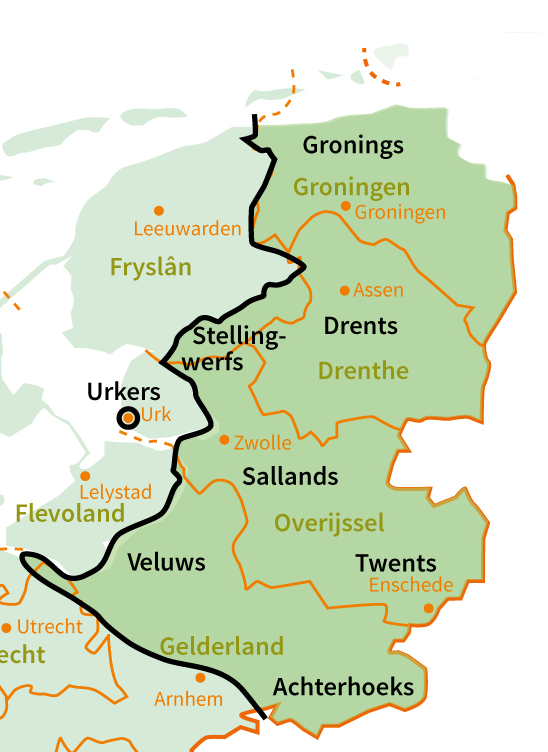
\includegraphics[height=.6\textheight]{Sekeres Fig 1.png}
    \caption{\label{fig:mapls}Map of the Low Saxon language area in the Netherlands (from \citealt{bloemhoff_introduction_2020})}   
\end{figure}

Whereas most dialects spoken in the Netherlands as well as Standard Dutch are descendants of Old Low Franconian \citep{de_schutter_dutch_1994}, the Low Saxon dialects descend from Old Saxon \citep{bloemhoff_handboek_2008}. This historical difference is still refelected in the way the dialects cluster nowadays, with Low Franconian and Low Saxon forming  distinct clusters \citep{nerbonne_phonetic_1996} and with Low Saxon displaying a relatively large distance towards Standard Dutch \citep{wielingEtAl2011b}. Speakers of Low Saxon in the Netherlands generally also speak (Standard) Dutch, as it is necessary to participate in all aspects of society such as education and interaction with more formal organisations. This has also contributed to the stark age-grading in speakers, with a relatively small number of young people speaking Low Saxon dialects \citep{bloemhoff_taalsociologische_2008}.

The Low Saxon dialect spoken in most of the area under investigation is Gronings. This label includes the dialects spoken in the northern part of Drenthe, as they are more closely related to dialects spoken in Groningen than the dialects spoken in the rest of Drenthe \citep{bloemhoff_introduction_2020}. Gronings is different from other dialects in the Netherlandic Low Saxon language area because of its Frisian substrate \citep{reker_talige_2008}, which is as of now most visible in diminutive formation with /k/ rather than /t/ after vowels, labials, /s/ and /r/ but without umlaut, as opposed to dialects in Drenthe and Twente, respectively (cf.  \citealt{van_bree_frisian_2017}), and because it did not (or only to a lesser degree) undergo Westphalian breaking, a sound change involving diphthongisation that resulted in a variety of pronunciations in the Westphalian dialects \citep{bloemhoff_introduction_2020}. Some of the most characteristic features of Gronings -- although not present in all varieties -- are the use of the diphthongs   
/ɑɪ/ and /ɔu/ (for example, in the words /lɑɪf/ `sweet' (of a person) and /bɔuk/ `book') where other Low Saxon variants have monophthongs such as /i/ or  /eː/ (/lif/ or /leːf/) and  /u/ or /oː/ (/buk/ or /boːk/) respectively \citep{reker_talige_2008}. 

\subsection{Research question and hypothesis}
This study investigates whether the framework and methods of cognitive geography can be usefully employed in dialectological research. Concretely, this is done by answering the question of whether including cognitive distance, in addition to geographic distance, leads to better predictions of perceptual dialect distance in the Gronings dialect area. Based on the cognitive geographic theory that mental representations of space are more influential in determining behaviour than space itself, we hypothesise that cognitive distances will add to geographic distance in predicting perceptual dialect distance. More specifically, we expect that an increase in cognitive distance leads to an increase in perceptual dialect distance (regardless of geographic distance), as cognitive distances can also represent the mental distance that a person feels towards a place which in turn might be tied to the distance they feel towards a dialect. Thus, the study sheds more light on the individual experience of space and how this is connected to the experience of language, drawing a parallel between perceptual dialectology and cognitive geography.

\section{Method}
\subsection{Participants}
A total of 1,034 participants from the provinces of Drenthe and Groningen participated in the study through an online survey. Participants who did not provide perceptual dialect distance estimates were removed, as well as participants who either indicated in the control question that they were not able to hear the dialect recordings sufficiently to provide the estimates or who did not answer the control question at all. This resulted in 789 remaining participants. Most of the participants were self-reported dialect speakers, with 96.2\% of the participants indicating that they were able to speak their local dialect to at least some degree, and 62.2\% of the participants indicating that they were able to effortlessly participate in any kind of conversation in their dialect. All but one of the participants indicated that they could understand their local dialect to at least some degree, and 74.4\% indicated that they were able to effortlessly understand anything in the dialect, even when spoken at a fast pace. The age of the participants ranged from 12 to 95, with a mean age of 49 and a standard deviation of 16. A total of 55.1\% of the participants identified as women, 43.9\% as men and 1\% preferred not to disclose their gender identity or identified as a non-binary gender. 

\subsection{Materials}
The survey was implemented in \citet{qualtrics_qualtrics_2005} and consisted of three sections: demographic questions (as discussed under the previous section, in addition to the location in which the participants grew up), cognitive distance estimates, and perceptual dialect distance estimates. The assessment of dialect proficiency (speaking skill and listening skill) was done through self-assessment: participants were asked to rate how well they were able to speak and understand their local dialect on a seven-point Likert scale. For the cognitive distance questions, participants were asked to estimate the distance from the place in which they grew up to seven places in Drenthe and Groningen (namely, Eelde, Finsterwolde, Grijpskerk, Onstwedde, Slochteren, Uithuizen, and Zevenhuizen). The speaker locations as well as the locations in which participants grew up can be found in \figref{fig:map}. These seven locations were selected because dialect recordings with identical speech from dialect speakers from these locations were already available from an earlier study on dialect change in the continental part of the Dutch language area \citep{heeringa_convergence_2014}. The recordings we used were the first five sentences of a text read aloud by one male speaker over 60 years of age per location, resulting in recordings of between 13 and 25 seconds. These texts were created by two to four of these speakers per location who wrote a consensus translation of a Dutch text, accompanied by movie stills. Because of the nature of the task, the recordings contained substantial lexical and stylistic variation. For each location, a recording was available of an older male and a younger female speaker. We chose to use the recordings from the older male speakers as these were further removed from the Dutch standard language \citep{heeringa_convergence_2014} and we therefore expected them to contain more readily identifiable dialect features. For the perceptual dialect distance estimates, participants were asked to listen to the associated dialect recordings (without knowing that these recordings came from the seven places mentioned earlier) and indicate to what degree they were similar to the dialect that was spoken in the place in which they grew up on a seven-point Likert scale, ranging from 1 (not alike at all) to 7 (very alike). Participants were presented with each recording once, but could replay them as often as necessary and had unlimited time to provide their estimate of similarity. The order of the recordings was the same for every participant, namely alphabetically arranged by speaker location. The survey was conducted in Dutch.

\begin{figure}
    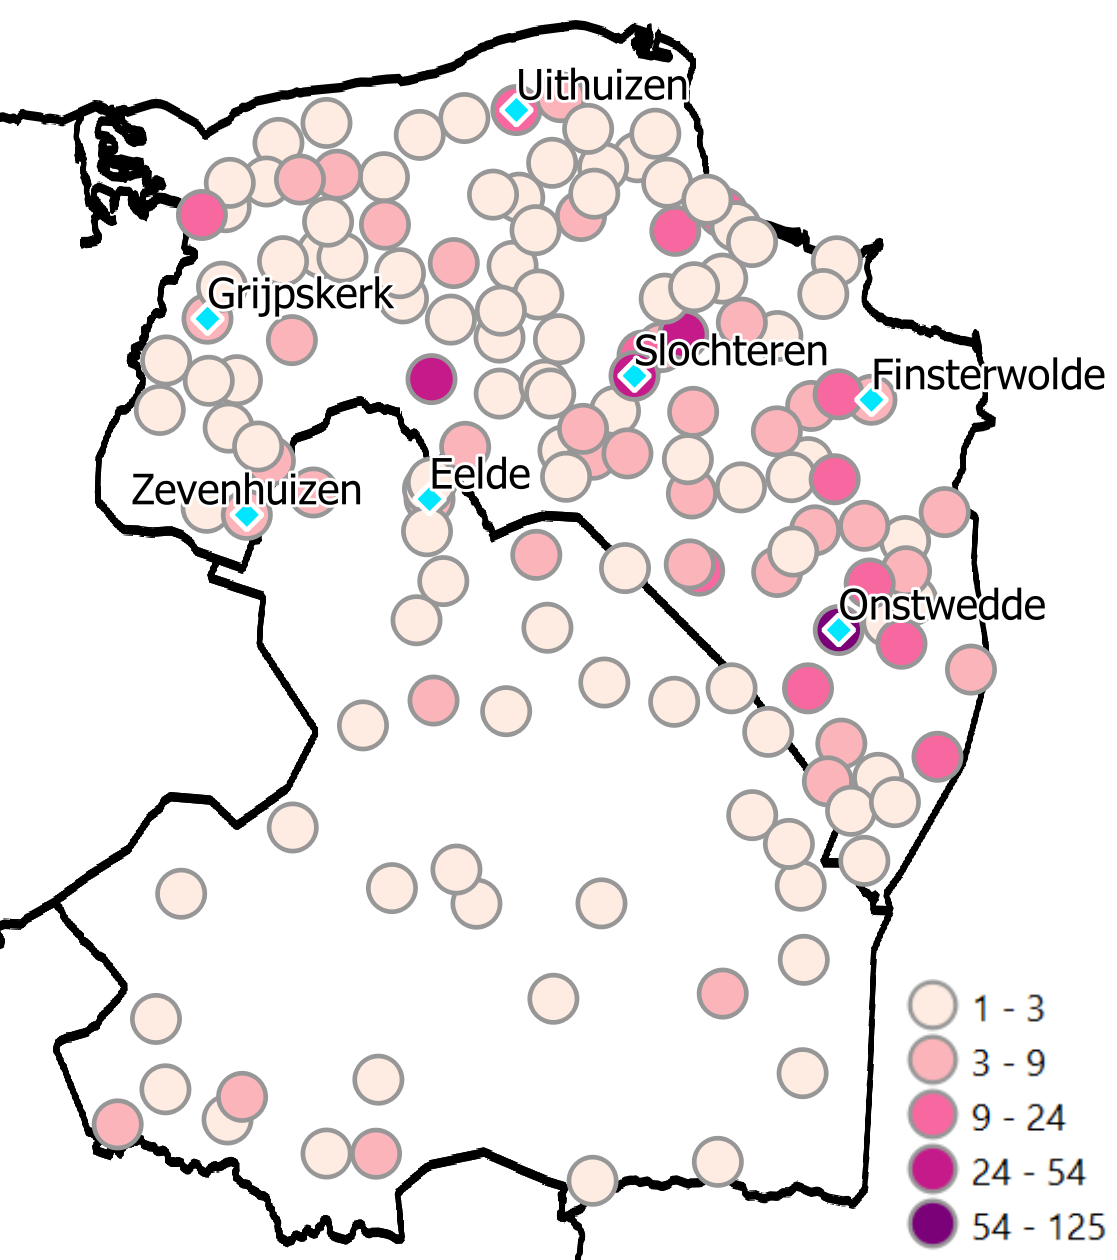
\includegraphics[width = \textwidth]{figures/sekeres/map_clean_legend2.png}
    \caption{Map of Groningen and Drenthe with the speaker locations (blue diamonds) and the participant locations (pink circles, with darker colours indicating a larger number of participants)}
    \label{fig:map}
\end{figure}
\newpage

\subsection{Procedure}
The survey was shared on the online platform of Centrum Groninger Taal \& Cultuur, a dialect organisation for Gronings, through social media and through the researchers' own networks. The topic of the study was not fully disclosed to participants. Instead they were informed that the study investigated dialects and regional languages in Drenthe and Groningen and that they would be asked to answer questions about locations in this area and listen to recordings. No compensation was provided for participating in the study. Ethical approval for this study was obtained from the Research Ethics Committee of the Faculty of Arts at the University of Groningen (CETO, reference number 81837041).

\subsection{Analysis}
A linear mixed-effects regression model was fitted to the data, using the \texttt{lme4} package \citep{bates_fitting_2015} in R \citep{r_core_team_r:_2020}. Three variables that possibly could account for random variation in the data were included in the model. Subject was included as a random-effect factor as the participants in this study were sampled from a larger possible set of participants. Subject location largely overlapped with subject, but was included as a separate random-effect factor as the set of locations from which a subset was taken for this study was not the same as the population from which the participants were selected. Finally, speaker location was included as a random-effect factor because the dialect recordings were selected from a potentially larger set of locations.\footnote{Note that including speaker location as a random effect is done here because the nature of this study is methodological. If the goal of the study was to investigate differences between the dialects of these locations, they would be included as a fixed effect.} As the effect that cognitive distance had on the estimation of dialect distance differed per subject, a by-subject random slope for cognitive distance was added. Similarly, the effect of geographic distance on the estimate of dialect distance differed per speaker location, so a by-speaker location random slope for geographic distance was added. The numeric variables (cognitive distance, geographic distance and birth year) were centered and scaled (i.e., $z$-transformed) to provide a better model fit and facilitate interpretation as the coefficients then reflect the relative size of the effects. Model comparison (using likelihood ratio tests) was used to identify which fixed and random effects it was necessary to include.

\section{Results}
\subsection{Hypothesis testing}
The model we used to test our hypothesis consisted of the fixed effects cognitive distance and geographic distance.\footnote{We also ran two versions of this model containing only cognitive distance and only geographic distance in order to test whether it was really the combination of the two factors that was effective and not just one of them. These models did not outperform the regular hypothesis model.} As indicated before, we took the structural variability of our data into account by including a random intercept for subject, subject location and speaker location, a by-subject random slope for cognitive distance and a by-speaker location random slope for geographic distance. All of these random effects were necessary, as they improved the model according to the likelihood ratio tests. This model thus tested the hypothesis that cognitive distance can partly (i.e., in addition to geographical distance) predict perceptual dialect distance. The fixed effect coefficients for this model can be found in \tabref{tab:fec_min}, and the random effects structure can be found in \tabref{tab:res_min}. Following \citet{nerbonne_measuring_2010}, we investigated whether the logarithm of the geographic distance was a better predictor of perceptual dialect distances than assuming a linear relationship, but this did not appear to be the case. The residuals of the final model followed a normal distribution, and autocorrelation and heteroskedasticity fell within normal bounds. A trimmed version of the model in which outliers (i.e., residuals that were more than 2.5 standard deviations away from the mean) were removed showed that the results were robust, i.e., not caused by outliers.  

\begin{table}
 \begin{tabular}{lcc S[table-format=2.3] S[table-format=1.2e-2] @{~}l }
  \lsptoprule
                 & {Estimate} & {Std. Error}  & {$t$} & {$p$} & \\
  \midrule
    Intercept           & 3.58283 & 0.28158 & 12.724 & 8.04e-06 & ***\\
    Geographic distance & 0.52906 & 0.07392 & 7.157 & 1.49e-02 & * \\
    Cognitive distance  & 0.09792 & 0.04016 & 2.438 & 5.85e-05 & ***\\
  \lspbottomrule
 \end{tabular}
\caption{Fixed effect coefficients of a minimal model for predicting perceptual dialect distance}
\label{tab:fec_min}
\end{table}

\begin{table}
\caption{Random effect structure of a minimal model for predicting perceptual dialect distance}
\label{tab:res_min}
 \begin{tabular}{llrrr}
  \lsptoprule
    Random-effect factor & Intercept/Slopes & Variance & Std. Dev. & Corr.\\
  \midrule
    Subject	& Intercept	& 0.56921  & 0.7545 & \\  	
     & Cognitive distance & 0.06672 & 0.2583 & 0.38\\
    Sbj.~location & Intercept & 0.17954 & 0.4237 & \\	
    Spk.~location & Intercept & 0.53213 & 0.7295	& \\
     & Geographic distance & 0.02684 & 0.1638 & 0.90\\
     Residual & & 1.73765 & 1.3182 & \\
  \lspbottomrule
 \end{tabular}
\end{table}

The hypothesis-testing model indicates that the predictor with the strongest effect on perceptual dialect distance (as estimated by the participants listening to dialect recordings) is geographic distance, as it has the highest estimate out of both $z$-transformed predictors. Larger geographical distances between places are associated with larger perceptual dialect distances. The effect of cognitive distance is less strong, but goes in the same direction: the further away participants believe a place is, the larger the perceptual dialect distance. 

\subsection{Exploratory analysis}
For the exploratory model, predictors were added step by step and were only included in consecutive models if they significantly improved the model, which was evaluated using model comparison. The set of potential predictors that were considered were cognitive distance, geographic distance, participant listening skill, participant speaking skill, participant gender, participant birth year, interactions between cognitive distance and geographic distance, between cognitive distance and listening skill, between cognitive distance and speaking skill, between cognitive distance and gender, between gender and listening skill, between gender and speaking skill as well as the random effects described above. Main effects and interactions were added to the model in this order, based on how likely they were estimated to have an effect following previous literature. In the final model, predictors with low $t$-values (i.e., lower than 2) were re-evaluated and removed from the model if model comparison indicated that including each of these predictors did not significantly improve the model compared to a model without that predictor. 
The fixed effect coefficients for this model can be found in \tabref{tab:fec_exp}, and the random effects structure can be found in \tabref{tab:res_exp}. In the final model, the residuals followed a normal distribution and both autocorrelation and heteroskedasticity fell within normal bounds. A trimmed version of the model in which outliers that were more than 2.5 standard deviations away from the mean were removed was run as well in order to assess whether the model was carried by outliers, which was not the case. 

\begin{table}
\caption{Fixed effect coefficients of an exploratory model for predicting perceptual dialect distance}
\label{tab:fec_exp}
\tabcolsep=.9\tabcolsep
 \begin{tabular}{l S[table-format=-1.5] S[table-format=1.5] S[table-format=-2.3] S[table-format=1.2e2, table-align-exponent=false] l}
  \lsptoprule
    & {Est.} & {SE}  & {$t$} & {$p$} & \\
  \midrule
    Intercept & 5.13280 & 0.37622 & 13.643 & 2.25e-11 & ***\\
    Cognitive distance & 0.10632 & 0.03998 & 2.660 & 0.007907 & **\\
    Geographic distance	& 0.49770 & 0.07559 & 6.584 & 0.000123 & ***\\
    Listening skill & -0.17891 & 0.06446 & -2.775 & 0.005647 & ** \\
    Speaking skill & -0.14201 & 0.03716 & -3.822 & 0.000144 & ***\\
    Gender (female vs.\ male)	& -0.18418 & 0.06643 & -2.772 & 0.005705 & **\\
    Cognitive distance & -0.06082 & 0.02158 & -2.818 & 0.005036 & **\\
    Geographic distance	& & & & & \\
  \lspbottomrule
 \end{tabular}
\end{table}

\begin{table}
\caption{Random effect structure of an exploratory model for predicting perceptual dialect distance}
\label{tab:res_exp}
 \begin{tabular}{lrrrc}
  \lsptoprule
    Random-effect factor & Intercept/Slope & Variance & Std. Dev. & Corr. \\
  \midrule
    Subject	& Intercept	& 0.52090 & 0.7217 & \\  	
     & Cognitive distance & 0.05919  & 0.2433  & 0.48\\
    Sbj.~location & Intercept & 0.12852 & 0.3585 & \\	
    Spk.~location & Intercept & 0.54786 & 0.7402	& \\
     & Geographic distance & 0.02820 & 0.1679 & 0.94\\
     Residual & & 1.74861 & 1.3224 & \\
  \lspbottomrule
 \end{tabular}
\end{table}

For the main effects, we now find an interaction between geographic distance and cognitive distance. The effect of cognitive distance is positive, but it is strongest when geographic distance is short, i.e., when the speaker location and the participant location are closer together. \figref{fig:interaction} visualizes this pattern. 

In addition, gender contributes to the model, with female participants providing lower perceptual dialect distances. Furthermore, an increase in speaking skill and listening skill (as gauged through self-assessment by the participants) corresponds to a decrease in perceived dialect distances. 

\begin{figure}
    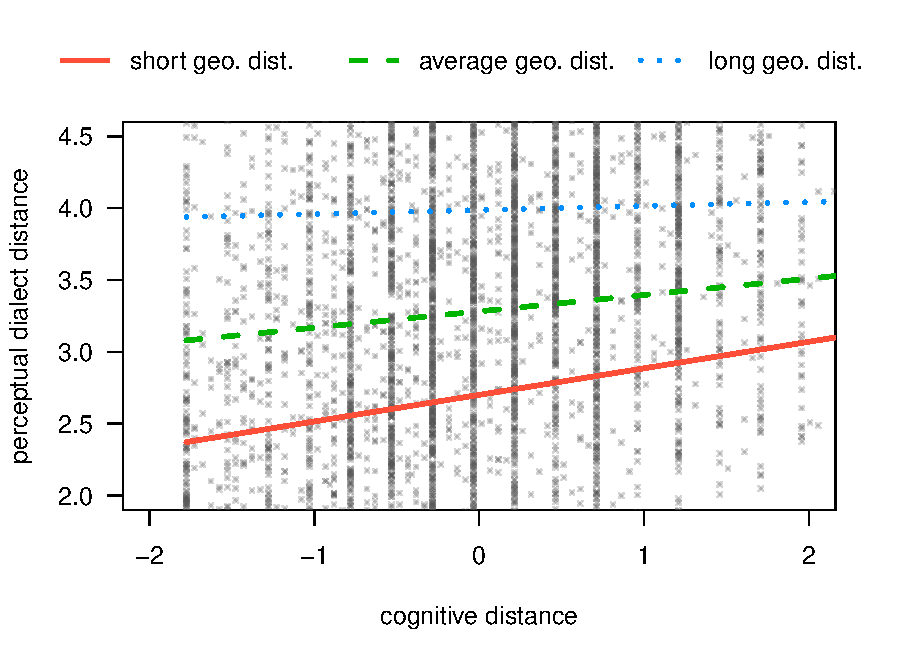
\includegraphics[width=\textwidth]{plot_newest.pdf}
    \caption{The interaction between cognitive distance and geographic distance in an exploratory model for predicting perceptual dialect distance. The crosses indicate the partial residuals.}
    \label{fig:interaction}
\end{figure}

\section{Discussion}
\subsection{General}
The research question of this study was whether cognitive distances could be used, in addition to geographic distance, to explain perceptual dialect distances. In our analysis, we first built a model to test our basic hypothesis and consecutively built an exploratory model to investigate other factors that might contribute to predicting perceptual dialect distances. The hypothesis-testing model revealed that cognitive distance does contribute to predicting perceptual dialect distance, as an increase in cognitive distance was related to an increase in perceptual dialect distance. Our initial hypothesis was thus confirmed. However, the effect of geographic distance was more predictive of differences in perceptual dialect distance than cognitive distance was. In contrast to earlier research assessing the relationship between geographic and dialect distances in large datasets \citep{heeringa_validating_2002}, the logarithm of geographic distance did not provide a better fitting model than simple linear geographic distance did.  This may have been caused by the relatively small geographic area that was under investigation \citep{heeringa_geographic_2007}.

Our exploratory analysis revealed an interaction between cognitive and geographic distance, in which the predictive value of cognitive distances was greater for smaller geographic distances. As people are better at predicting distances towards locations they are familiar with \citep{day_urban_1976, montello_measurement_1991}, it is not surprising that cognitive distance is more predictive for locations that participants are closer to geographically. Geographic distance, however, does not necessarily have a direct relation to familiarity, so it could be beneficial for future studies to separately measure the degree of familiarity between participants and the locations. The relationship between cognitive and geographic distance indicates that the use of cognitive distance in dialect research might be especially useful for studying small geographical areas. In this case, the provinces of Groningen and Drenthe, which span a combined 5,640 km$^2$, already represent a relatively large geographical area for a study on cognitive distances.
 
Three additional predictors for perceptual dialect distance were significant in the exploratory model. First, both an increase in speaking skill and listening skill were connected to a lower perceptual dialect distance. An effect of dialect proficiency could unfold in two ways. Either more familiarity with the dialect could lead to lower perceptual distances in general, or more familiarity could lead to a better ability to distinguish the different dialects which in turn leads to higher perceptual distances. In this case, it appears that higher proficiency in each skill leads to lower perceived dialect distances. This could be caused by the composition of our sample which was relatively biased toward highly proficient users of dialect: 62.2\% of participants indicated that they were able to effortlessly participate in any kind of conversation in their dialect and 74.4\% indicated that they were able to effortlessly understand anything in the dialect, even when spoken at a fast pace. It could be possible that familiarity with the dialect leads to lower perceptual distances up to a certain degree and that only people who are very familiar with the dialects can use this familiarity to better distinguish among them. A more balanced study design with more people who are not proficient or have only limited proficiency in their local dialect could provide more insight in this finding.

Second, women in general provided lower perceptual dialect distances than men. This result might seem unexpected, as men, or more specifically non-mo\hyp bile, older, rural males or NORMs, are usually seen as more proficient dialect speakers \citep{chambers_dialectology_1980}, and familiarity might lower the perceptual ratings. Welch two sample \textit{t}-tests revealed that the men in the sample did indeed report significantly higher speaking and listening skills than the women. However, no significant interaction between gender and either listening skill or speaking skill was found in the exploratory model, making this explanation unlikely. Studies on the effect of listener gender (rather than speaker gender) on dialect classification are sparse, but one study on regional variants in Turkey found found that men distinguished more different dialect areas than women did \citep{demirci_gender_2002}. However, as the author mentions, this could also be an effect that is specific to a context in which women have less access to education and social institutions. Future research would have to determine whether robust differences in listener gender exist in estimating perceptual dialect distances.

\subsection{Limitations}
As the recordings used in this study came from a pre-existing dataset, the choice of locations was rather limited. In the area under investigation, only seven locations were available out of which five were very small, having fewer than 3,000 inhabitants. Therefore, not all participants may have been familiar with every location they were asked to provide a distance estimate for. Although the random intercept for speaker location partly compensates for this, it would be better for future studies to only incorporate locations that are likely to be known to all or most of the participants, for example by conducting a pre-test. Furthermore, an assessment of cultural prominence \citep{montgomery_effect_2012} could provide additional information on how these locations might be represented in the minds of participants.

Additionally, some participants indicated in the survey that they found it difficult to specify a single place where they grew up, for example because they spent their youth in several locations, or because a large part of their social life took place in a different location than where they lived. Other aspects of mobility that could influence dialect perception or the estimates of cognitive distance are locations where participants did not grow up but where they lived for a significant part of their adult life, locations where they worked, the location(s) where their parents grew up or locations they were otherwise familiar with. These relations to other locations were not captured by the survey used in this study, but could provide interesting additional insight for future studies. Gathering more information on mobility patterns and the familiarity that participants have with different locations (see \citealt{JeszenszkyEtAl2024}) could improve both our understanding of the cognitive distance estimates that participants provided and the perceptual dialect distances they reported.

\subsection{Broader implications and future research}
Within the field of dialectology, space is usually treated as a relatively static variable, rather than as an environment in which people move around and which they experience. We have attempted to incorporate this experience of space in dialectology, in the same way that the experience of language has been incorporated in the field through perceptual dialectology. Earlier endeavours to incorporate techniques from (cultural) geography in dialectological research and perceptual dialectology in particular have greatly improved our understanding of the relationship between language, space and culture. The use of cognitive geographic techniques expands the toolbox of dialectologists by offering new explanations for the perception of language variation in a manner that is cognitively informed.

In our study, cognitive distance estimates served as the quantification of the experience of space. These distances contributed to the prediction of perceptual dialect distance, especially when geographic distance was short. The effect of cognitive distance on perceptual dialect distance in our model displayed a large amount of variation per subject, as cognitive distance is a highly individual measure. Nonetheless, it seems that the aggregate analysis that was used was suitable for our study, as individual and demographic differences between participants could be taken into account. Although there was a clear effect of cognitive distance, it does appear that this type of analysis is especially useful when smaller areas are considered than was done in this study. However, the area under investigation cannot be too small either as there would still need to be a sufficient amount of linguistic diversity in the geographic sense. Perhaps a collection of villages on the border of two language areas or neighbourhoods within a large city would be suitable places for a similar study, as they allow for a relatively high amount of language variation within a geographically small area. In these cases, and especially for a study in an urban environment, the linguistic variants under investigation could also be socially stratified (in addition to their spatial stratification) in order to further assess to what degree the cognitive distances are different from pure geographic distances. Furthermore, an analysis that is more focused on individual linguistic and geographic behaviour could provide more insight into the exact relation between the experience of space and the experience of language. 

The results of this study show that the framework and methods of cognitive geography can be usefully employed in the field of (especially perceptual) dialectology. Although the aggregate nature of our study makes it difficult to assess what the relationship between language and space in the mind entails exactly, we have provided a first glimpse into the possible use of cognitive geography in the field of dialectology. As the current study is methodological in nature, the dialect areas under investigation served as a test case. In future research, this approach can now be used to conduct studies in which the dialects themselves take a more central focus.

\section{Conclusion}
In this study, we have attempted to answer the question of whether the framework and methods from the field of cognitive geography could be usefully employed in dialectological research. This was done through a study that investigated the effect of cognitive distances on perceptual dialect distances in Groningen and Drenthe. The results of this study indicate that it is indeed the case that the framework and methods from cognitive geography can be used in dialectological research. This opens up new directions of research in which the human experience of space is used to explain linguistic phenomena. 



% \is{Cognition} %add "Cogntion" to subject index for this page


\section*{Contributions}
Hedwig Sekeres contributed to conceptualisation, methodology, formal analysis, investigation, and writing -- original draft.
Martijn Wieling contributed to conceptualisation, writing -- review \& editing, and supervision.
Remco Knooihuizen contributed to writing -- review \& editing.

\sloppy
% here we change the meaning of \VAN to use the prefix for the bibliography
%\DeclareRobustCommand{\VAN}[3]{#3}
\printbibliography[heading=subbibliography,notkeyword=this]
\end{document}
